% !TeX spellcheck = cs_CZ
%{\tikzset{external/prefix={tikz/FYZII/}}
% \tikzset{external/figure name/.add={ch25_}{}}
%---------------------------------------------------------------------------------------------------
% file fey2ch25.tex
%---------------------------------------------------------------------------------------------------
%=========================== Kapitola Elektrodynamika v relativistickém zápisu =====================
\setchaptertoc
\chapter{Elektrodynamika v relativistickém zápisu}\label{fyz:IIchapXXV}

  \section{Čtyřvektory}\label{fyz:IIchapXXVsecI}
  \section{Skalární součin}\label{fyz:IIchapXXVsecII}
  \section{Čtyřrozměrný gradient}\label{fyz:IIchapXXVsecIII}
  \section{Elektrodynamika v čtyřrozměrném zápisu}\label{fyz:IIchapXXVsecIV}
  \section{Čtyřpotenciál pohybujícího se náboje}\label{fyz:IIchapXXVsecV}
  \section{Invariance rovnic elektrodynamiky}\label{fyz:IIchapXXVsecVI}
  \section{Příklady a cvičení}\label{fyz:IIchapXXVsecVII}

    \begin{figure}[ht!] %\ref{fyz:fig600}
      \centering
      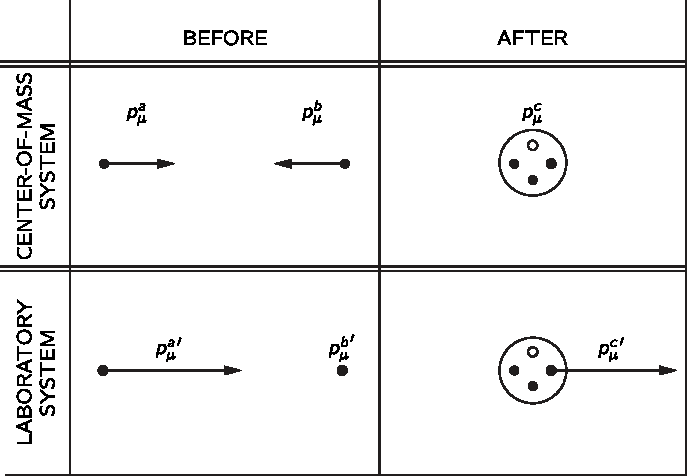
\includegraphics[width=0.7\linewidth]{fyz_fig600.pdf}
      \caption{
               (\cite[s.~707]{Feynman02})}
      \label{fyz:fig600}
    \end{figure}


    \begin{figure}[ht!] %\ref{fyz:fig601}
      \centering
      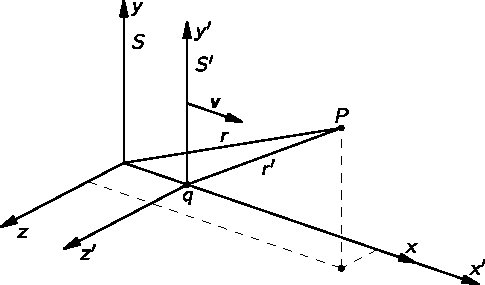
\includegraphics[width=0.7\linewidth]{fyz_fig601.pdf}
      \caption{
               (\cite[s.~707]{Feynman02})}
      \label{fyz:fig601}
    \end{figure}
    
    \todo[inline]{Kapitola fey2ch25 je nedodělaná, obsahuje pouze obrázky}
%} %tikzset
%---------------------------------------------------------------------------------------------------